\begin{figure}
 \centering
 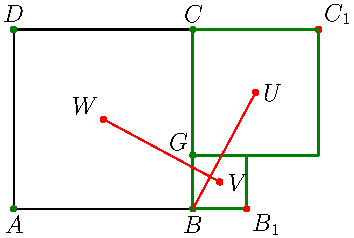
\includegraphics{./Ccomp16_1.pdf}
 % Ecomp16_1.pdf: 0x0 pixel, 300dpi, 0.00x0.00 cm, bb=
 \caption{Calcul des affixes.}
 \label{fig:Ccomp16_1}
\end{figure}

\begin{enumerate}
 \item Le calcul de $c$ et $d$ ne pose pas de problème : $c = 1+i$, $d = i$.\newline
 On obtient les centres des carrés comme milieux de sommets opposés :
\begin{displaymath}
 w = \frac{1}{2}(a+c) = \frac{1}{2} + \frac{1}{2}i.
\end{displaymath}
Pour le calcul de $u$ et $v$, on introduit les points $B_1$ avec $b_1 = b +\gamma$ et $C_1$ avec $c_1 = c + (1-\gamma)$ (figure \ref{fig:Ccomp16_1}).
\begin{align*}
 u &= \frac{1}{2}(g+c_1)
 = \frac{1}{2}(1+\gamma i + 1 + i + (1-\gamma))
 = \frac{3-\gamma}{2} + \frac{1+\gamma}{2}i \\
v &= \frac{1}{2}(g + b_1)
 = \frac{1}{2}(1+\gamma i + 1 + \gamma)
 = \frac{2 + \gamma}{2} + \frac{\gamma}{2}i
\end{align*}

\item Calculons les affixes des vecteurs $\overrightarrow{UB}$ et $\overrightarrow{VW}$.
\begin{displaymath}
\left. 
\begin{aligned}
 b - u &= \frac{-1+\gamma}{2} - \frac{1+\gamma}{2}i \\
 w - v &= -\frac{1+\gamma}{2} + \frac{1-\gamma}{2}i
\end{aligned}
\right\rbrace 
\Rightarrow
i(w-v) = b-u
\end{displaymath}
Les segments $UB$ et $VW$ sont donc orthogonaux et de même longueur.
\end{enumerate}
